% Options for packages loaded elsewhere
\PassOptionsToPackage{unicode}{hyperref}
\PassOptionsToPackage{hyphens}{url}
%
\documentclass[
  12 pt,
]{article}
\usepackage{amsmath,amssymb}
\usepackage{lmodern}
\usepackage{setspace}
\usepackage{ifxetex,ifluatex}
\ifnum 0\ifxetex 1\fi\ifluatex 1\fi=0 % if pdftex
  \usepackage[T1]{fontenc}
  \usepackage[utf8]{inputenc}
  \usepackage{textcomp} % provide euro and other symbols
\else % if luatex or xetex
  \usepackage{unicode-math}
  \defaultfontfeatures{Scale=MatchLowercase}
  \defaultfontfeatures[\rmfamily]{Ligatures=TeX,Scale=1}
\fi
% Use upquote if available, for straight quotes in verbatim environments
\IfFileExists{upquote.sty}{\usepackage{upquote}}{}
\IfFileExists{microtype.sty}{% use microtype if available
  \usepackage[]{microtype}
  \UseMicrotypeSet[protrusion]{basicmath} % disable protrusion for tt fonts
}{}
\makeatletter
\@ifundefined{KOMAClassName}{% if non-KOMA class
  \IfFileExists{parskip.sty}{%
    \usepackage{parskip}
  }{% else
    \setlength{\parindent}{0pt}
    \setlength{\parskip}{6pt plus 2pt minus 1pt}}
}{% if KOMA class
  \KOMAoptions{parskip=half}}
\makeatother
\usepackage{xcolor}
\IfFileExists{xurl.sty}{\usepackage{xurl}}{} % add URL line breaks if available
\IfFileExists{bookmark.sty}{\usepackage{bookmark}}{\usepackage{hyperref}}
\hypersetup{
  pdftitle={ECON30520: Final Project on Beauty dataset},
  pdfauthor={Nikita Fernes - 18205420},
  hidelinks,
  pdfcreator={LaTeX via pandoc}}
\urlstyle{same} % disable monospaced font for URLs
\usepackage[margin=1in]{geometry}
\usepackage{color}
\usepackage{fancyvrb}
\newcommand{\VerbBar}{|}
\newcommand{\VERB}{\Verb[commandchars=\\\{\}]}
\DefineVerbatimEnvironment{Highlighting}{Verbatim}{commandchars=\\\{\}}
% Add ',fontsize=\small' for more characters per line
\usepackage{framed}
\definecolor{shadecolor}{RGB}{248,248,248}
\newenvironment{Shaded}{\begin{snugshade}}{\end{snugshade}}
\newcommand{\AlertTok}[1]{\textcolor[rgb]{0.94,0.16,0.16}{#1}}
\newcommand{\AnnotationTok}[1]{\textcolor[rgb]{0.56,0.35,0.01}{\textbf{\textit{#1}}}}
\newcommand{\AttributeTok}[1]{\textcolor[rgb]{0.77,0.63,0.00}{#1}}
\newcommand{\BaseNTok}[1]{\textcolor[rgb]{0.00,0.00,0.81}{#1}}
\newcommand{\BuiltInTok}[1]{#1}
\newcommand{\CharTok}[1]{\textcolor[rgb]{0.31,0.60,0.02}{#1}}
\newcommand{\CommentTok}[1]{\textcolor[rgb]{0.56,0.35,0.01}{\textit{#1}}}
\newcommand{\CommentVarTok}[1]{\textcolor[rgb]{0.56,0.35,0.01}{\textbf{\textit{#1}}}}
\newcommand{\ConstantTok}[1]{\textcolor[rgb]{0.00,0.00,0.00}{#1}}
\newcommand{\ControlFlowTok}[1]{\textcolor[rgb]{0.13,0.29,0.53}{\textbf{#1}}}
\newcommand{\DataTypeTok}[1]{\textcolor[rgb]{0.13,0.29,0.53}{#1}}
\newcommand{\DecValTok}[1]{\textcolor[rgb]{0.00,0.00,0.81}{#1}}
\newcommand{\DocumentationTok}[1]{\textcolor[rgb]{0.56,0.35,0.01}{\textbf{\textit{#1}}}}
\newcommand{\ErrorTok}[1]{\textcolor[rgb]{0.64,0.00,0.00}{\textbf{#1}}}
\newcommand{\ExtensionTok}[1]{#1}
\newcommand{\FloatTok}[1]{\textcolor[rgb]{0.00,0.00,0.81}{#1}}
\newcommand{\FunctionTok}[1]{\textcolor[rgb]{0.00,0.00,0.00}{#1}}
\newcommand{\ImportTok}[1]{#1}
\newcommand{\InformationTok}[1]{\textcolor[rgb]{0.56,0.35,0.01}{\textbf{\textit{#1}}}}
\newcommand{\KeywordTok}[1]{\textcolor[rgb]{0.13,0.29,0.53}{\textbf{#1}}}
\newcommand{\NormalTok}[1]{#1}
\newcommand{\OperatorTok}[1]{\textcolor[rgb]{0.81,0.36,0.00}{\textbf{#1}}}
\newcommand{\OtherTok}[1]{\textcolor[rgb]{0.56,0.35,0.01}{#1}}
\newcommand{\PreprocessorTok}[1]{\textcolor[rgb]{0.56,0.35,0.01}{\textit{#1}}}
\newcommand{\RegionMarkerTok}[1]{#1}
\newcommand{\SpecialCharTok}[1]{\textcolor[rgb]{0.00,0.00,0.00}{#1}}
\newcommand{\SpecialStringTok}[1]{\textcolor[rgb]{0.31,0.60,0.02}{#1}}
\newcommand{\StringTok}[1]{\textcolor[rgb]{0.31,0.60,0.02}{#1}}
\newcommand{\VariableTok}[1]{\textcolor[rgb]{0.00,0.00,0.00}{#1}}
\newcommand{\VerbatimStringTok}[1]{\textcolor[rgb]{0.31,0.60,0.02}{#1}}
\newcommand{\WarningTok}[1]{\textcolor[rgb]{0.56,0.35,0.01}{\textbf{\textit{#1}}}}
\usepackage{longtable,booktabs,array}
\usepackage{calc} % for calculating minipage widths
% Correct order of tables after \paragraph or \subparagraph
\usepackage{etoolbox}
\makeatletter
\patchcmd\longtable{\par}{\if@noskipsec\mbox{}\fi\par}{}{}
\makeatother
% Allow footnotes in longtable head/foot
\IfFileExists{footnotehyper.sty}{\usepackage{footnotehyper}}{\usepackage{footnote}}
\makesavenoteenv{longtable}
\usepackage{graphicx}
\makeatletter
\def\maxwidth{\ifdim\Gin@nat@width>\linewidth\linewidth\else\Gin@nat@width\fi}
\def\maxheight{\ifdim\Gin@nat@height>\textheight\textheight\else\Gin@nat@height\fi}
\makeatother
% Scale images if necessary, so that they will not overflow the page
% margins by default, and it is still possible to overwrite the defaults
% using explicit options in \includegraphics[width, height, ...]{}
\setkeys{Gin}{width=\maxwidth,height=\maxheight,keepaspectratio}
% Set default figure placement to htbp
\makeatletter
\def\fps@figure{htbp}
\makeatother
\setlength{\emergencystretch}{3em} % prevent overfull lines
\providecommand{\tightlist}{%
  \setlength{\itemsep}{0pt}\setlength{\parskip}{0pt}}
\setcounter{secnumdepth}{5}
\usepackage{float}
\usepackage{booktabs}
\usepackage{siunitx}
\newcolumntype{d}{S[input-symbols = ()]}
\usepackage{longtable}
\usepackage{array}
\usepackage{multirow}
\usepackage{wrapfig}
\usepackage{colortbl}
\usepackage{pdflscape}
\usepackage{tabu}
\usepackage{threeparttable}
\usepackage{threeparttablex}
\usepackage[normalem]{ulem}
\usepackage{makecell}
\usepackage{xcolor}
\ifluatex
  \usepackage{selnolig}  % disable illegal ligatures
\fi
\newlength{\cslhangindent}
\setlength{\cslhangindent}{1.5em}
\newlength{\csllabelwidth}
\setlength{\csllabelwidth}{3em}
\newenvironment{CSLReferences}[2] % #1 hanging-ident, #2 entry spacing
 {% don't indent paragraphs
  \setlength{\parindent}{0pt}
  % turn on hanging indent if param 1 is 1
  \ifodd #1 \everypar{\setlength{\hangindent}{\cslhangindent}}\ignorespaces\fi
  % set entry spacing
  \ifnum #2 > 0
  \setlength{\parskip}{#2\baselineskip}
  \fi
 }%
 {}
\usepackage{calc}
\newcommand{\CSLBlock}[1]{#1\hfill\break}
\newcommand{\CSLLeftMargin}[1]{\parbox[t]{\csllabelwidth}{#1}}
\newcommand{\CSLRightInline}[1]{\parbox[t]{\linewidth - \csllabelwidth}{#1}\break}
\newcommand{\CSLIndent}[1]{\hspace{\cslhangindent}#1}

\title{ECON30520: Final Project on Beauty dataset}
\author{Nikita Fernes - 18205420}
\date{18 January, 2022}

\begin{document}
\maketitle

\setstretch{1.5}
\hypertarget{introduction}{%
\section{Introduction}\label{introduction}}

This paper will study the impact of an instructor's appearance on their course evaluation. Our main dependent variable of interest is course evaluation \emph{eval} which is on a scale of 1 to 5 and our main explanatory variable is \emph{beauty} that is averaged across a panel of 6 students. Overall, we have 9 explanatory variables 4 of which are numeric and the rest categorical. First we have some descriptive statistics, then we introduce some relationships between the variables and finally we perform a multiple regression using OLS to estimate the effect of beauty of course evaluation.

\hypertarget{literature-review}{%
\section{Literature Review}\label{literature-review}}

A study by Ponzo and Scoppa (2012) done in an Italian university with a fairly large data set shows that beauty does in fact have a significant positive correlation with course evaluation even in an intellectual profession such as teaching. They also state that beauty in this profession may be more important for females than for males.

However, the magnitude of this correlation is much lower in a German study by Süssmuth (2006) where the impact of overall beauty in the instructor's course evaluation is positive but only significant at a 10\% level of significance in one group of younger students. There was no significant relationship with the other groups of students. An interesting point to note is that Süssmuth (2006) found that courses taught in English had better instructional ratings showcasing that language can have a great impact on course evaluation. They also found that there was some indication of gender discrimination by advanced students.

\hypertarget{descriptive-statistics}{%
\section{Descriptive Statistics}\label{descriptive-statistics}}

\hypertarget{numerical-variables}{%
\subsection{Numerical Variables}\label{numerical-variables}}

To start with we describe the numerical data in the table given below. Here, we see that the average teaching evaluation score is 4 out of 5 which seems to be quite good considering it is above average. The beauty rating that is averaged across the panelists was shifted to have a mean of 0 as seen in the table. Average age of an instructor is 48 and the mean number of students in a course is 55.

\begin{tabular}{l|l}
\hline
 & study (N = 463)\\
\hline
\bf{Overall teaching evaluation score} & ~\\
\hline
~~ min & 2.1\\
\hline
~~ max & 5\\
\hline
~~ mean (sd) & 4.00 $\pm$ 0.55\\
\hline
\bf{Beauty rating of instructor by 6 students} & ~\\
\hline
~~ min & -1.450494\\
\hline
~~ max & 1.970023\\
\hline
~~ mean (sd) & 0.00 $\pm$ 0.79\\
\hline
\bf{Age of instructor} & ~\\
\hline
~~ min & 29\\
\hline
~~ max & 73\\
\hline
~~ mean (sd) & 48.37 $\pm$ 9.80\\
\hline
\bf{Number of students in course} & ~\\
\hline
~~ min & 8\\
\hline
~~ max & 581\\
\hline
~~ mean (sd) & 55.18 $\pm$ 75.07\\
\hline
\end{tabular}

\newpage

\hypertarget{categorical-variables}{%
\subsection{Categorical Variables}\label{categorical-variables}}

Most of our categorical variables are binary variables so I have combined them with one another and some numerical variables to get a more in depth and stylised analysis of the data. This part of the paper deals with the features of the instructor.

We have a pie chart that shows us the number of minority professors, separated by gender. We see that in a total of 195 females, 36 belong to a minority background and 159 do not i.e., they are caucasian. Again, in a total of 268 males only 28 are from minority backgrounds. This shows that there is a majority of males as well as caucasian instructors.

\begin{figure}[H]

{\centering 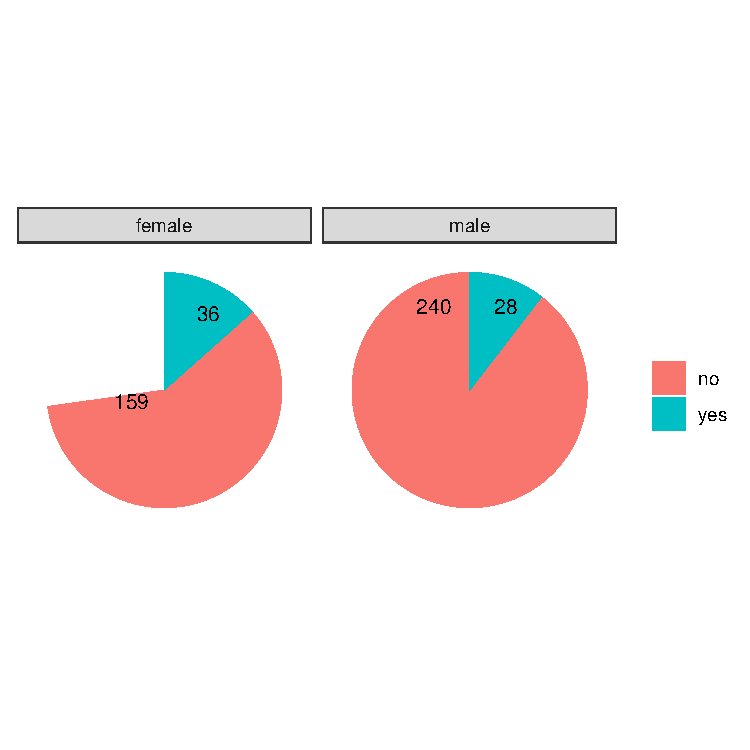
\includegraphics{18205420_Markdown--1-_files/figure-latex/piechart-1} 

}

\caption{Pie chart of minority professors by gender}\label{fig:piechart}
\end{figure}
\newpage

Next, we have a simple histogram paired with a density plot that smoothes out the the distribution of age using a kernel density estimate. We see as before the age distribution is largely concentrated in the 48-50 range same as the mean previously described. `we also see some concentration around the 58-60 age group followed by 35-37 year olds.

\begin{figure}[H]

{\centering 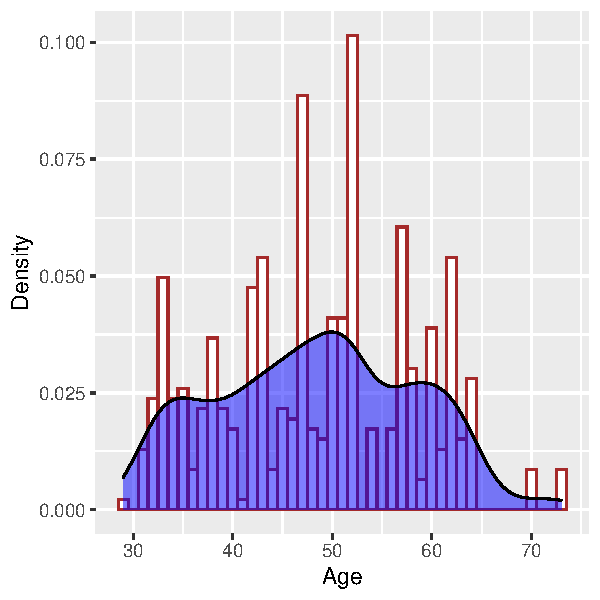
\includegraphics{18205420_Markdown--1-_files/figure-latex/histogram-1} 

}

\caption{Histogram by age}\label{fig:histogram}
\end{figure}
\newpage

Here, I wanted to see the relationship between the beauty rating with gender and whether the instructor was a native english speaker. We already know that the mean of beauty is 0 that is easily noticeable in this violin plot. However, we see that native speakers overall have a higher beauty rating, more for women than for men. Important to note from the graph that females that are non-native english speakers have more negative averaged beauty ratings than males that are non-native english speakers. However, overall females have a higher beauty rating as well showing that perhaps females as instructors are more criticized for their looks.

\begin{figure}[H]

{\centering 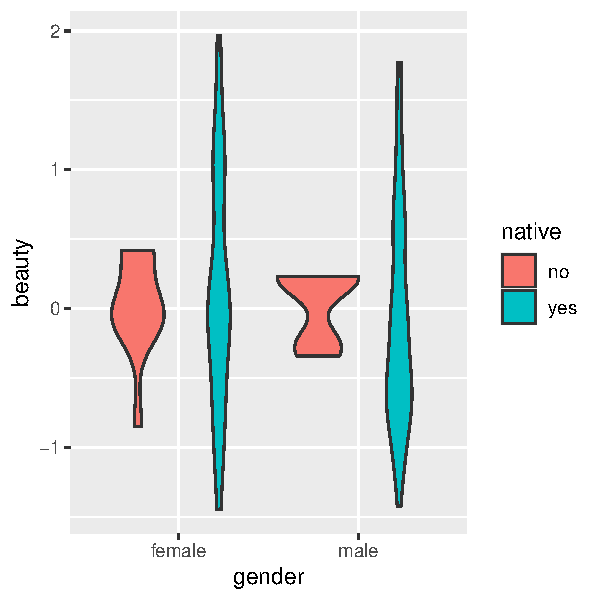
\includegraphics{18205420_Markdown--1-_files/figure-latex/violin-1} 

}

\caption{Violin plot of age by Gender, separated by native}\label{fig:violin}
\end{figure}
\newpage

\hypertarget{relationships-with-evaluation}{%
\section{Relationships with evaluation}\label{relationships-with-evaluation}}

Just like the relationship seen before with beauty and gender we will be looking at some relationships with evaluation which is the main dependent variable.
In the boxplot below in figure \ref{fig:boxplot} we see that native english speakers have a higher average in course evaluation than non-native speakers. The whiskers that represent the confidence intervals also differ in both groups.

\begin{figure}[H]

{\centering 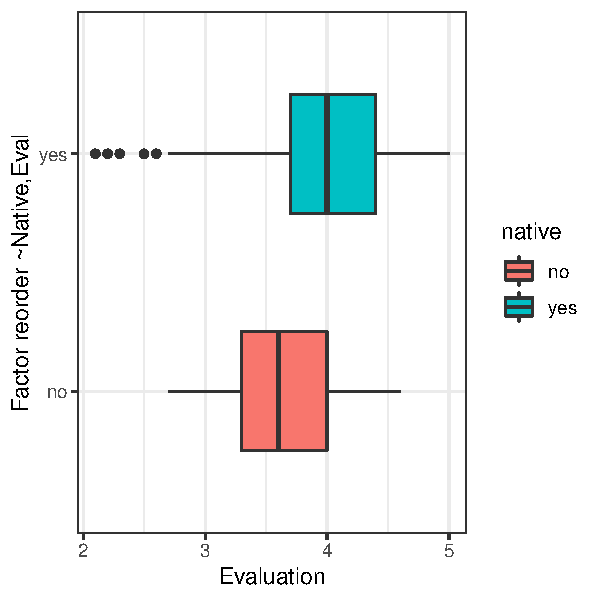
\includegraphics{18205420_Markdown--1-_files/figure-latex/boxplot-1} 

}

\caption{Boxplot showing evaluation if native or not}\label{fig:boxplot}
\end{figure}

\newpage

In the relationship below in figure \ref{fig:rel1} we regress evaluation on beauty however we further distinguish the two by the type of course i.e., whether it is a single-credit elective or not. The graph below shows us that when the course is not a single credit elective, beauty and evaluation have a positive correlation. In contrast, when the course is a single credit elective beauty and evaluation have a negative correlation.

\begin{figure}[H]

{\centering 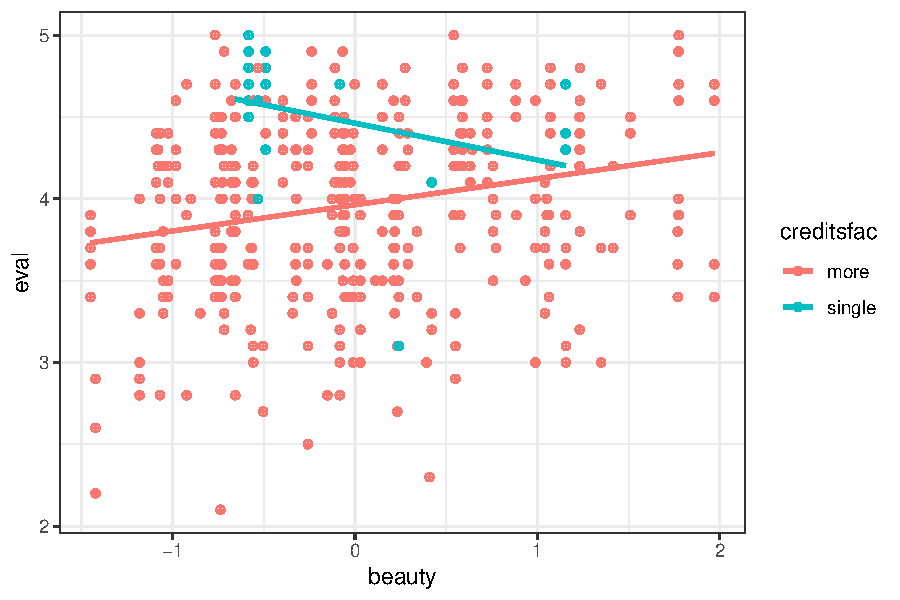
\includegraphics{18205420_Markdown--1-_files/figure-latex/rel1-1} 

}

\caption{Scatter plot of evaluation on beauty separated by credits}\label{fig:rel1}
\end{figure}

\newpage

Here in figure \ref{fig:rel2} we see how course evaluation on beauty differs in a lower division versus in a upper division course, wherein lower division consist mainly of freshmen and sophomores whereas upper division consists largely of seniors. Using the following graph we can see that in the lower division the correlation between beauty and evaluation begins as positive however after a few fluctuations it shows a negative correlation when beauty is rated above 0.5.
Upper division also shows one fluctuation in the correlation between beauty and evaluation however overall it has a positive relationship as with an increase in beauty there is an increase in course evaluation.

\begin{figure}[H]

{\centering 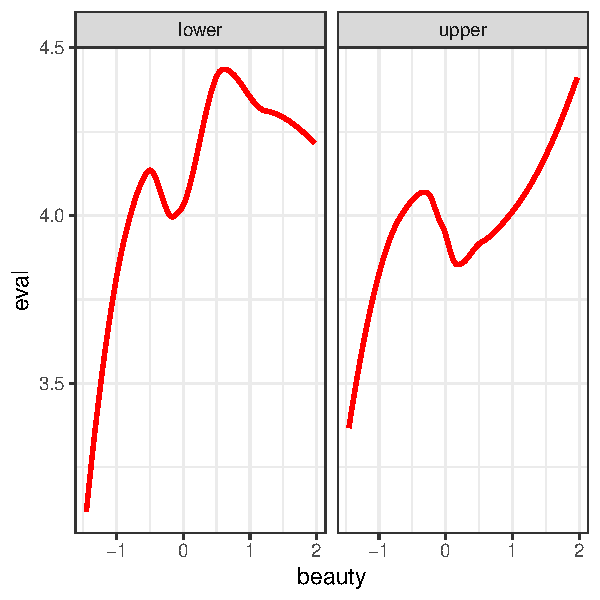
\includegraphics{18205420_Markdown--1-_files/figure-latex/rel2-1} 

}

\caption{Relationship of evaluation on beauty separated by division that is ordered by age}\label{fig:rel2}
\end{figure}
\newpage

This relationship below in figure \ref{fig:rel3} shows us how tenure affects the relationship between course evaluation and beauty. We see a positive relationship between beauty and evaluation for instructors that have tenure as well as those that don't. At a glance it seems that they run parallel to one another and may have the similar if not the same slopes. For those without tenure, the evaluation seems to be higher at every level of beauty rating.

\begin{figure}[H]

{\centering 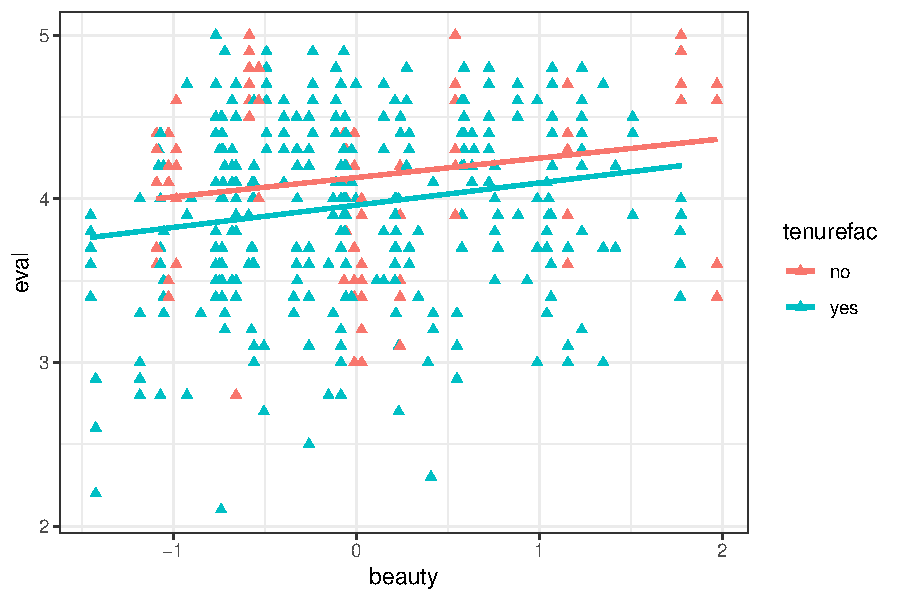
\includegraphics{18205420_Markdown--1-_files/figure-latex/rel3-1} 

}

\caption{Course evaluation on beauty separated by Tenure}\label{fig:rel3}
\end{figure}

\newpage

This final graph \ref{fig:rel4} showcases the distribution of age and gender as we regress our dependent variable = evaluation on our main explanatory variable = beauty.
We see an overall positive correlation between beauty and course evaluation, the relationship of which we will be looking in depth in the next segment. This graph makes it easy for us to see that female instructors are given a higher beauty rating than men as we observe on the right side of the graph. Another point to note is that when beauty \textgreater{} 0, the age groups seem to be of a younger cohort of instructors.

\begin{figure}[H]

{\centering 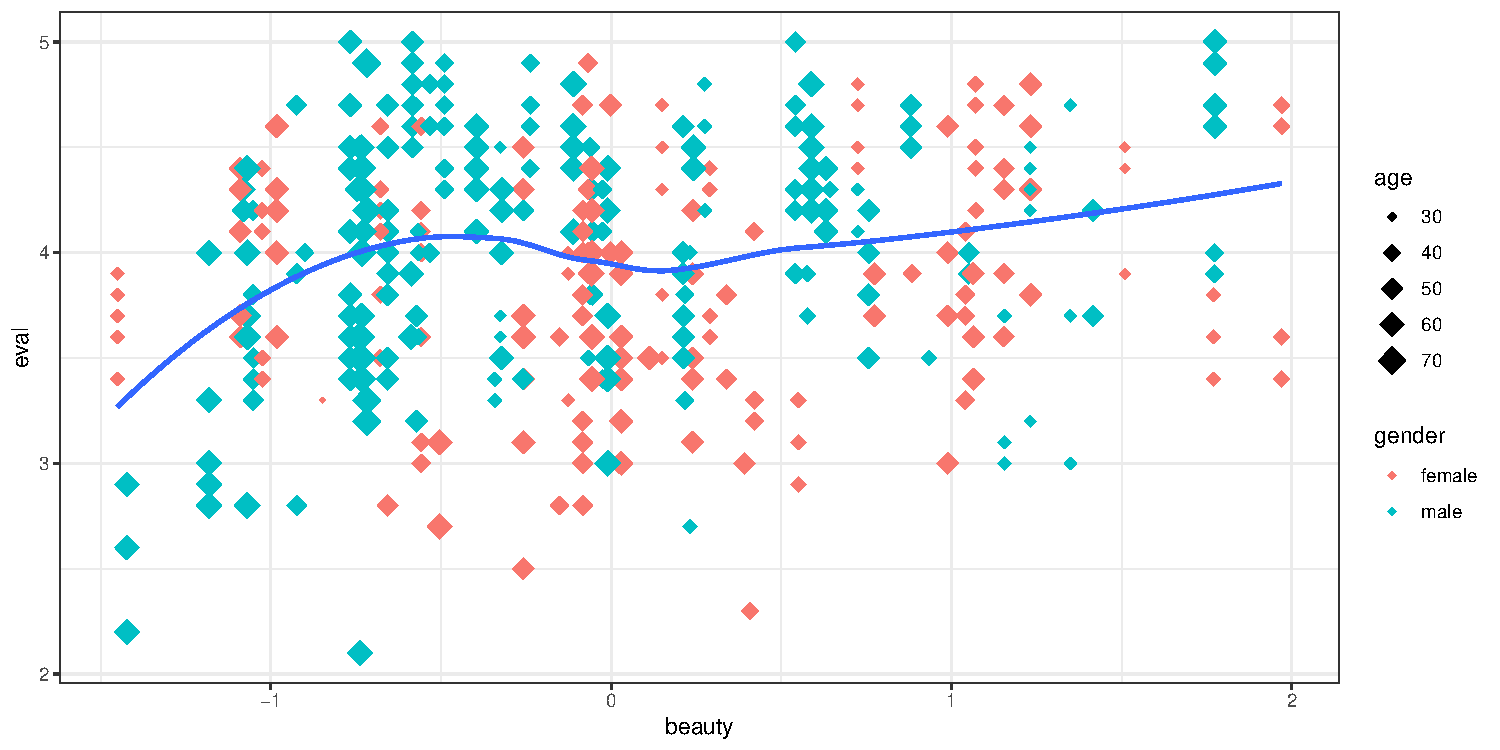
\includegraphics{18205420_Markdown--1-_files/figure-latex/rel4-1} 

}

\caption{Scatter plot with age and gender, regressing beauty on evaluation}\label{fig:rel4}
\end{figure}

Looking into gender further, we see in figure \ref{fig:rel5} that beauty has a higher impact on evaluation of male instructors than females which is contrary to the findings of Ponzo and Scoppa (2012) where beauty for females has a greater impact.

\begin{figure}[H]

{\centering 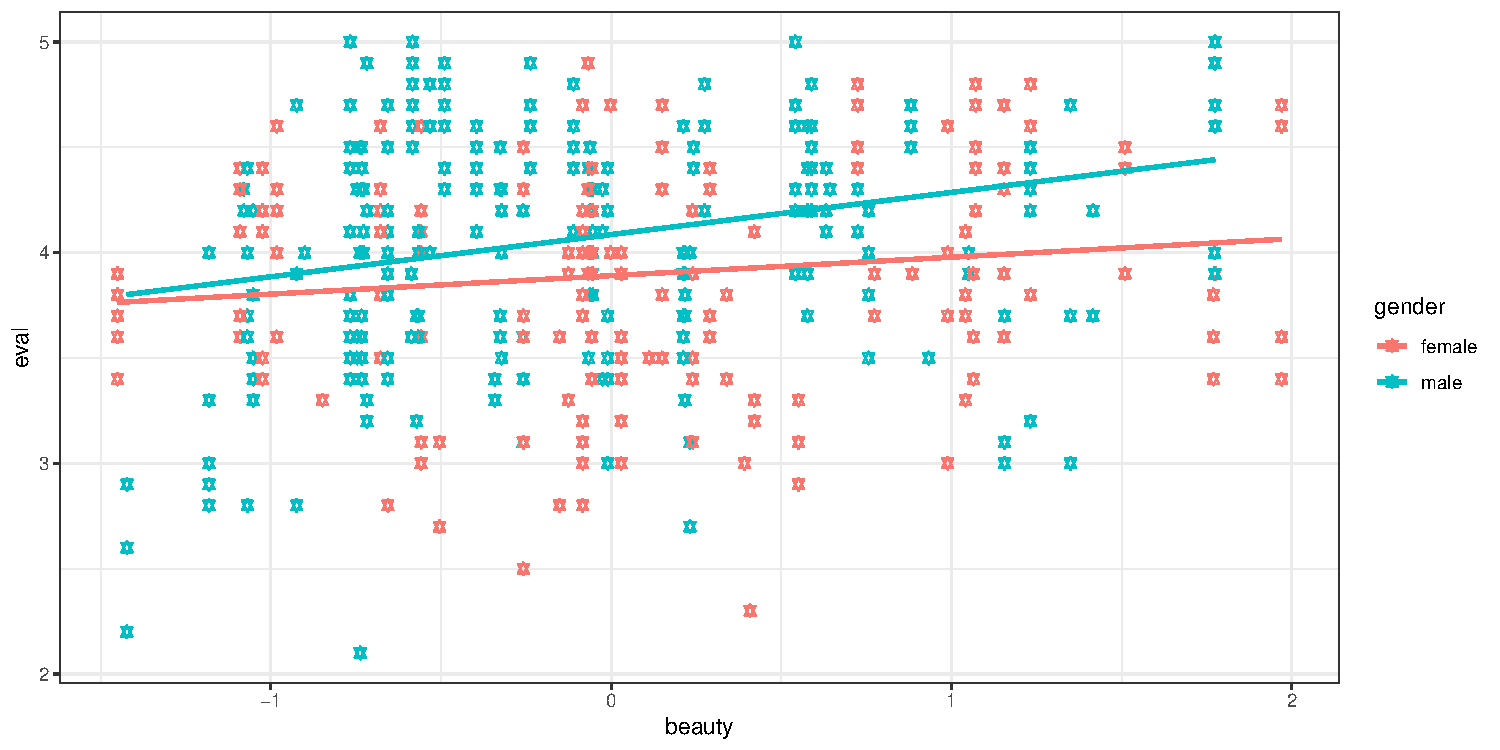
\includegraphics{18205420_Markdown--1-_files/figure-latex/rel5-1} 

}

\caption{Evaluation on beauty, by gender}\label{fig:rel5}
\end{figure}

\hypertarget{regressions}{%
\section{Regressions}\label{regressions}}

\hypertarget{ordinary-least-squares}{%
\subsection{Ordinary Least Squares}\label{ordinary-least-squares}}

Using all the information above we create a regression to check if there exists a significant correlation between the explanatory and dependent variable - course evaluation \emph{eval}. I have done 1 simple regression between evaluation and beauty which was previously plotted in figure \ref{fig:rel4} as well as 2 multiple regressions.

\begin{Shaded}
\begin{Highlighting}[]
\NormalTok{lm\_main}\OtherTok{=} \FunctionTok{lm}\NormalTok{(eval}\SpecialCharTok{\textasciitilde{}}\NormalTok{beauty, }\AttributeTok{data=}\NormalTok{study)}

\NormalTok{lm\_professor }\OtherTok{=} \FunctionTok{lm}\NormalTok{(study}\SpecialCharTok{$}\NormalTok{eval }\SpecialCharTok{\textasciitilde{}}\NormalTok{ study}\SpecialCharTok{$}\NormalTok{beauty }\SpecialCharTok{+}\NormalTok{ study}\SpecialCharTok{$}\NormalTok{age }\SpecialCharTok{+} 
\NormalTok{           study}\SpecialCharTok{$}\NormalTok{gender }\SpecialCharTok{+}\NormalTok{ study}\SpecialCharTok{$}\NormalTok{minority }\SpecialCharTok{+}\NormalTok{study}\SpecialCharTok{$}\NormalTok{native, study)}

\NormalTok{lm\_mult }\OtherTok{=} \FunctionTok{lm}\NormalTok{(study}\SpecialCharTok{$}\NormalTok{eval }\SpecialCharTok{\textasciitilde{}}\NormalTok{ study}\SpecialCharTok{$}\NormalTok{beauty }\SpecialCharTok{+}\NormalTok{ study}\SpecialCharTok{$}\NormalTok{age }\SpecialCharTok{+} 
\NormalTok{           study}\SpecialCharTok{$}\NormalTok{gender }\SpecialCharTok{+}\NormalTok{ study}\SpecialCharTok{$}\NormalTok{minority}\SpecialCharTok{+}\NormalTok{study}\SpecialCharTok{$}\NormalTok{native}\SpecialCharTok{+}
\NormalTok{           study}\SpecialCharTok{$}\NormalTok{division }\SpecialCharTok{+}\NormalTok{ study}\SpecialCharTok{$}\NormalTok{tenure }\SpecialCharTok{+}\NormalTok{ study}\SpecialCharTok{$}\NormalTok{credits}\SpecialCharTok{+}\NormalTok{study}\SpecialCharTok{$}\NormalTok{allstudents)}

\NormalTok{models}\OtherTok{\textless{}{-}}\FunctionTok{list}\NormalTok{(lm\_main,lm\_professor,lm\_mult,lm\_mult)}
\end{Highlighting}
\end{Shaded}

\[
eval = \beta_0 + \beta_1 beauty + \beta_2 age + \beta_3 gender +\beta_4 minority + \beta_5 native
\]
\[
\beta_6 division +\beta_7 tenure + \beta_8 credits + \beta_9 allstudents
\]

\begin{table}

\caption{\label{tab:reg1output}Regression Table}
\centering
\begin{tabular}[t]{lcccc}
\toprule
  & Main & Instructor & Overall & Robust\\
\midrule
beauty & \num{0.133} &  &  & \\
 & (\num{0.032}) &  &  & \\
 & {}[p = \num{0.000}] &  &  & \\
Beauty &  & \num{0.141} & \num{0.159} & \num{0.159}\\
 &  & (\num{0.033}) & (\num{0.032}) & (\num{0.031})\\
 &  & {}[p = \num{0.000}] & {}[p = \num{0.000}] & {}[p = \vphantom{1} \num{0.000}]\\
Age &  & \num{-0.003} & \num{-0.002} & \num{-0.002}\\
 &  & (\num{0.003}) & (\num{0.003}) & (\num{0.003})\\
 &  & {}[p = \num{0.325}] & {}[p = \num{0.381}] & {}[p = \num{0.381}]\\
Male &  & \num{0.207} & \num{0.195} & \num{0.195}\\
 &  & (\num{0.053}) & (\num{0.052}) & (\num{0.054})\\
 &  & {}[p = \num{0.000}] & {}[p = \num{0.000}] & {}[p = \num{0.000}]\\
Minority &  & \num{-0.044} & \num{-0.164} & \num{-0.164}\\
 &  & (\num{0.076}) & (\num{0.077}) & (\num{0.070})\\
 &  & {}[p = \num{0.558}] & {}[p = \num{0.034}] & {}[p = \num{0.034}]\\
Native speaker &  & \num{0.313} & \num{0.238} & \num{0.238}\\
 &  & (\num{0.109}) & (\num{0.108}) & (\num{0.101})\\
 &  & {}[p = \num{0.004}] & {}[p = \num{0.027}] & {}[p = \num{0.027}]\\
Upper-Division &  &  & \num{-0.015} & \num{-0.015}\\
 &  &  & (\num{0.057}) & (\num{0.059})\\
 &  &  & {}[p = \num{0.789}] & {}[p = \num{0.789}]\\
Tenure &  &  & \num{-0.058} & \num{-0.058}\\
 &  &  & (\num{0.063}) & (\num{0.060})\\
 &  &  & {}[p = \num{0.361}] & {}[p = \num{0.361}]\\
Credits &  &  & \num{0.587} & \num{0.587}\\
 &  &  & (\num{0.118}) & (\num{0.115})\\
 &  &  & {}[p = \num{0.000}] & {}[p = \num{0.000}]\\
No. of Students &  &  & \num{0.000} & \num{0.000}\\
 &  &  & (\num{0.000}) & (\num{0.000})\\
 &  &  & {}[p = \num{0.458}] & {}[p = \num{0.458}]\\
\midrule
Num.Obs. & \num{463} & \num{463} & \num{463} & \num{463}\\
R2 & \num{0.036} & \num{0.089} & \num{0.159} & \num{0.159}\\
Std.Errors & Classical & Classical & Classical & Robust\\
\bottomrule
\multicolumn{5}{l}{\rule{0pt}{1em}P-values in square brackets}\\
\multicolumn{5}{l}{\rule{0pt}{1em}In final column, robust standard errors in parentheses}\\
\multicolumn{5}{l}{\rule{0pt}{1em}Standard errors in parentheses}\\
\end{tabular}
\end{table}

In the \textbf{Main} regression, we see that as beauty increases by 1, eval increases by 0.13. As the p value os 0 we see that it is quite a string signifcant relationship at all the significant levels - \emph{1\%,5\% \& 10\%} The standard error is 0.032. The 95\% confidence interval is {[}b-2(0.032), b+2(0/032){]} and it has a very low R square.

In the second \textbf{Instructor} model that takes into account the attributes of the instructor we see that beauty, gender and native speaker are highly significant. The rest are statistically insignificant and therefore I do not feel the need to discuss them. Although, it is interesting to note how age has a negative correlation with evaluation though insignificant. Holding every other variable constant in each interpretation:
- As beauty increases by 1, evaluation increases by 0.14
- Being male increases the evaluation score by 0.206
- Being a native speaker, increases the evaluation score by 0.313
Overall R square has also increased to 0.89.

In the \textbf{Final} model, that includes all the given explanatory variables shows us that beauty, gender and credits are statistically significant at all levels of significance. Minority that was statistically insignificant before is not significant at the 5\% and 10\% levels of significance. In contrast, native speaker that was statistically significant at all levels before is now significant only at 5\% and 10\% levels. Upper-Division and Tenure are weakly significant at the 10\% level of significance. Age is still statistically insignificant. Holding others constant in each interpretation:
- As beauty increases by 1 unit eval increases by 0.159
- Being male increases the evaluation score by 0.195
- Increase in elective by 1 unit increases evaluation by 0.587
- Being a native speaker, increases the evaluation score by 0.238
- Being from a minority background decreases the evaluation score by 0.164
- Being an instructor in an upper-division course decreases the evaluation score by 0.015
- Being an instructor on tenure can decrease the evaluation score by 0.58

R square increases to 0.159 showing that this final model has a better goodness-of-fit than the other models. There is also a slight but notable difference in standard errors between the robust and classical model.

\hypertarget{coefficient-plots}{%
\subsection{Coefficient Plots}\label{coefficient-plots}}

The coefficient plot shows us the 95\% confidence intervals of all the coefficients. We see that at and number of students are 0 with no confidence intervals.

\begin{figure}[H]

{\centering 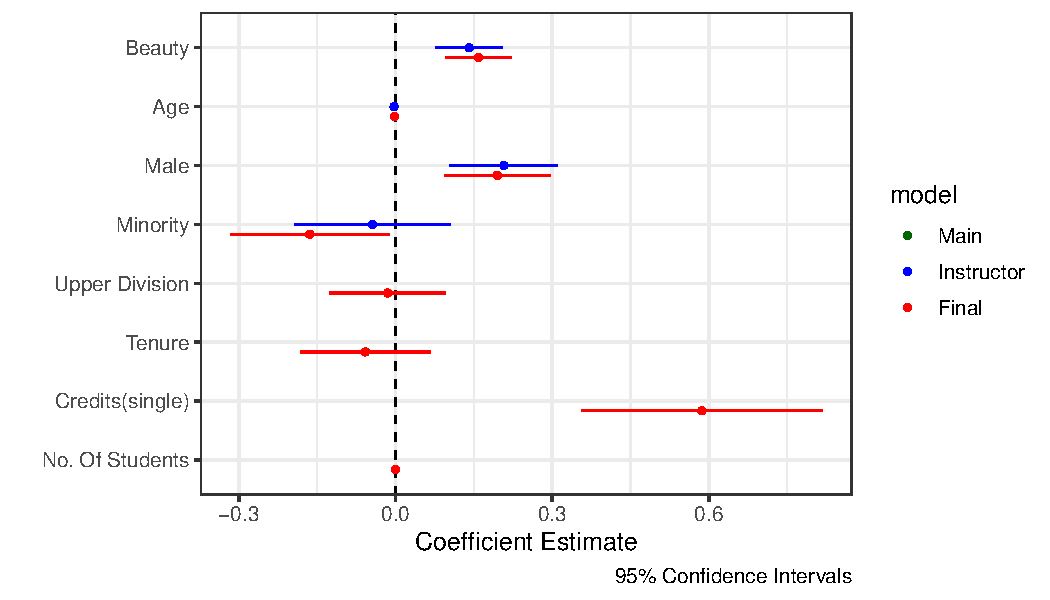
\includegraphics{18205420_Markdown--1-_files/figure-latex/coefplot-1} 

}

\caption{Coefficient Plot of OLS models}\label{fig:coefplot}
\end{figure}
\newpage

\hypertarget{conclusion}{%
\section{Conclusion}\label{conclusion}}

Overall we see that beauty is statistically significant in each model and therefore has a positive correlation with the evaluation of the course even while controlling for all other factors. This matches the study done in Italy by Ponzo and Scoppa (2012) as previously mentioned. The characteristics of the instructor that is out of his/her control that have an effect on this relationship is gender, being a native speaker and coming from a minority background. This is similar to what we see in the study in Germany by Süssmuth (2006) that shows us languages and gender can have an effect on evaluation. In terms of the course attributes that have nothing to do with beauty, being on tenure, teaching a single/multiple credit course and whether they teach an upper-division or lower-division course also have an impact on course evaluation.

\hypertarget{references}{%
\section*{References}\label{references}}
\addcontentsline{toc}{section}{References}

\hypertarget{refs}{}
\begin{CSLReferences}{1}{0}
\leavevmode\hypertarget{ref-Ref1}{}%
Ponzo, Michela, and Vincenzo Scoppa. 2012. {``The Good, the Bad, and the Ugly: Teaching Evaluations, Beauty and Abilities.''} \url{https://ideas.repec.org/p/clb/wpaper/201204.html}.

\leavevmode\hypertarget{ref-Ref2}{}%
Süssmuth, Bernd. 2006. {``Beauty in the Classroom: Are German Students Less Blinded? Putative Pedagogical Productivity Due to Professors' Pulchritude: Peculiar or Pervasive?''} \emph{Applied Economics} 38: 231--38.

\end{CSLReferences}

\end{document}
